\documentclass[10pt,a4paper]{article}
\usepackage[utf8]{inputenc}
\usepackage[english]{babel}
\usepackage{amsmath}
\usepackage{amsfonts}
\usepackage{amssymb}
\usepackage{graphicx}
\usepackage{float}
\title{Handwritten recognition neural network}
\author{Ladislav Petera}
\date{\today}
\begin{document}
\maketitle

\section{Introduction}

http://neuralnetworksanddeeplearning.com/chap1.html


\subsection{Perceptron}

Digital inputs and output:
\begin{itemize}
\item w - weight vector
\item x - input vector
\item b - threshold
\end{itemize}

$$ 
f(x_{i..j}) = 
\begin{cases} 
  0 & \text{if } w \cdot  x + b \leq 0  \\
  1 & \text{if } w \cdot x + b  > 0
\end{cases}
$$

\subsection{Sigmoid neurons}

Analog inputs and output

$$
output = \sigma(w \cdot x + b)
$$

$$
\sigma(z) = \frac{1}{1 + e^{-z}}
$$



\section{Network description}

\begin{figure}[H]
\centering
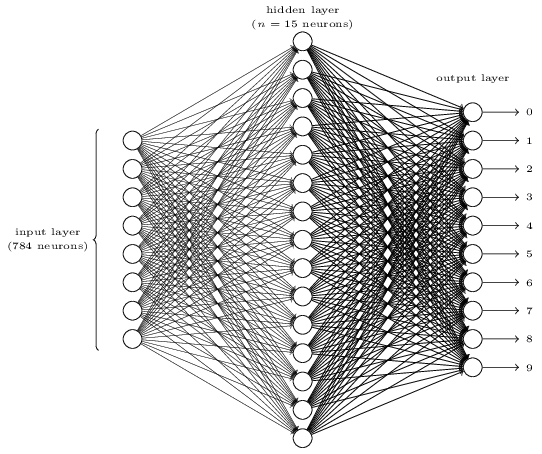
\includegraphics[width=10cm]{network-configuration.png}
\caption{Network configuration}
\end{figure}

\subsection{Network function:}

$$ y = y(x) $$

Where:

\begin{itemize}
\item x is the a 28 x 28 = 784-dimensional input vector (0.0 - 1.0 grayscale for each point)
\item y is the 10-dimensional output vector (0.0 - 1.0 "probability"" of being a given character)
\end{itemize}

\subsection{Quadratic cost function:}

$$ C(\omega, b) \equiv \frac{1}{2n} \sum_x || y(x) - a ||^2 $$

where:
\begin{itemize}
\item $\omega$ is vector of all weights in the network 
\item b denotes all the biases
\item n is total number of training inputs
\item a is the vector of outputs of the network when x is input
\item sum is over all training inputs x
\end{itemize}

\subsection{Gradient descent}

We are looking for the global minimum of the n-dimensional cost function.

Explanation in x of $R^2$:

\begin{figure}[H]
\centering
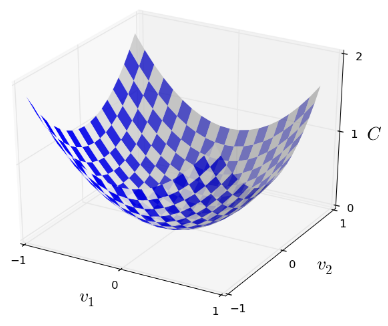
\includegraphics[width=10cm]{gradient.png}
\caption{Gradient}
\end{figure}

Let's imagine we have placed a ball on some position $v_1$, $v_2$ and look what happens when we move it by a small amount $\Delta v_1$ in direction $v_1$ and $\Delta v_2$ in direction $v_2$. C changes as follows:

$$ \Delta C \approx \frac{\delta C}{\delta v_1} \Delta v_1 + \frac{\delta C}{\delta v_2} \Delta v_2 $$

We are looking for a way to make $\Delta C$ negative (make tha ball roll down the valley). For this it helps to define $\Delta v$ to be vector of changes in v, $\Delta v \equiv (\Delta v_1, \Delta v_2)^T$ where T is te transpose operation, turning row vectors into column vectors. We denote the gradient vector by $\nabla C$ i.e.:

$$ \nabla C \equiv (\frac{\delta C}{\delta v_1},\frac{\delta C}{\delta v_2}) $$

With this the change in C can also be rewritten as:

$$ \Delta C \approx \nabla C \cdot \Delta v $$

This equations helps us choose $\Delta v$ as to make $\Delta C$ negative. Let's suppose we  choose
$$
\Delta v = -\eta \nabla C
$$
where $\eta$ is a small, positive parameter (known as learning rate). 

From this follows:
$$ \Delta C \approx -\eta \nabla C \cdot \nabla C = -\eta || \nabla C ||^2$$

Because $|| \nabla C ||^2 \geq 0$, this guarantees that $\Delta C \leq 0$ i.e. C will always decrease, never increase, if we change v according to the prescription.

This gives us the equation of one step in a gradient descent:

$$ v \to v^, = v - \eta \nabla C $$

\subsection{Using gradient descent in learning of neural networks}

We are looking for weights $\omega_k$ and biases $b_l$ which minimize the cost $C(\omega, b)$

Rewriting the gradient descent update rule in terms of these components:
$$ \omega_k \to \omega_k^, = \omega_k - \eta\frac{\delta C}{\delta \omega_k} $$
$$ b_l \to b_l^, = b_l - \eta\frac{\delta C}{\delta b_l} $$

\subsection{Stochastic gradient descent}

\textbf{Challenge:}

C has the form of $C = \frac{1}{n}\sum_x C_x$ that is an average over costs $C_x \equiv \frac{||y(x)-a ||^2}{2}$ for individual training examples. In practice to compute the gradient $\nabla C$ we need to compute the gradients $\nabla C_x$ separately for each training input, x, and then average them, $\nabla C = \frac{1}{n}\sum_x\nabla C_x$. Unfortunately, when the number of training inputs is very large this can take a long time, and learning thus occurs slowly.

\textbf{Idea:}

Estimate the gradient $\nabla C$ by computing $\nabla C_x$ for a small sample of randomly chosen training inputs. By averaging over this small sample it turns out that we can quickly get a good estimate of the true gradient $\nabla C$, and this helps speed up gradient descent, and thus learning.

Main idea - randomly choose a small number of training inputs m (mini-batch):
$$ \frac{\sum_{j=1}^m \nabla C_{X_j}}{m} \approx \frac{\sum_x \nabla C_x}{n} = \nabla C$$

\subsection{Test data}

Learning and test database: http://yann.lecun.com/exdb/mnist/


\end{document}